Let \( \mathcal{D} \) denote a convex open set in $\mathbb{R}^3$ with boundary $\Gamma$ and $\hat{n}$ a unit vector normal to $\Gamma$ and pointing outwards of \( \mathcal{D} \).
The neutral-particle direction of motion is defined as the unit vector $\hat{\Omega}$ on the unit sphere $\mathcal{S} = \{ \hat{\Omega} \in \mathbb{R}^3:|\hat{\Omega}| = 1 \}$.
The incoming and outgoing boundaries are defined with respect to $\hat{\Omega}$ and the position vector $\Vec{r}$ as subsets of the boundary $\Gamma$ in the following manner, respectively:

\begin{equation}
\Gamma^- (\hat{\Omega}) = \{ \hat{r} \in \Gamma : \hat{\Omega} \cdot \hat{n}(\Vec{r}) < 0 \}
\end{equation}

\begin{equation}
\Gamma^+ (\hat{\Omega}) = \{ \hat{r} \in \Gamma : \hat{\Omega} \cdot \hat{n}(\Vec{r}) > 0 \}
\end{equation}

Given the above definitions it is now possible to define the following boundary value problem: find the angular flux $\psi ( \Vec{r}, \hat{\Omega} )$ that satisfies the steady-state, one-speed transport equation

\begin{equation} \label{eq:TE}
\hat{\Omega} \cdot \nabla \psi ( \Vec{r} , \hat{\Omega} ) + \sigma _T ( \Vec{r} ) \psi ( \Vec{r} , \hat{\Omega} ) = \frac{\sigma_s (\Vec{r})}{4 \pi} \Phi ( \Vec{r} ) + q ( \Vec{r} ) .
\end{equation}

In Eq. \ref{eq:TE} we assumed a non-multiplying medium with isotropic scattering, but these constraints are easy to relax.
Indeed the current version of \ac{THOR} is capable of modeling transport phenomena in multiplying media with anisotropic scattering.
Equation \ref{eq:TE} is supplemented with applicable boundary conditions of the standard form

\begin{equation}
    \psi ( \Vec{r} , \hat{\Omega} ) = \psi_{bc} ( \hat{\Omega} ) , \Vec{r} \in \Gamma^- ( \hat{\Omega} )
\end{equation}

\noindent where the total and scattering macroscopic cross-sections, $\sigma_T$ and $\sigma_s$, are assumed to be positive and constant across a material region such that the scattering ratio $c = \sigma_s / \sigma_T $ remains smaller than unity.
The \textit{scalar} flux is defined in terms of the angular flux such that

\begin{equation} \label{eq:scalarF}
    \Phi ( \Vec{r} ) = \int _{4 \pi} d \hat{\Omega } \psi ( \Vec{r} , \hat{\Omega } )
\end{equation}

\noindent where the integral over $\hat{\Omega }$ represents the contribution of the angular flux over all possible directions.
The fixed source $ q ( \Vec{r} )$ represents the contribution to the angular flux from particles emitted by the external source that implicitly include in the case of a multiplying media, contributions from fission events.

Two important assumptions regarding the model problem presented above.
First, the scattering from a given direction $\hat{\Omega} ' $ into another direction $\hat{\Omega}$ was assumed to be isotropic, implying an equal probability for particles emitted in a scattering event to appear in any direction.
However, \ac{THOR} accounts for anisotropic scattering in the standard fashion of expanding the scattering cross section's angular dependence in Legendre polynomials then using Legendre's Addition Theorem to write the angle-dependent scattering source in terms of angular moments of the flux.
These details are skipped here but are available to the novice reader in standard textbooks if needed~\cite{Lewis1993}.
Second, the model as written assumes that the flux has no energy dependence.
The addition of energy dependence to the angular flux, also known as the multi-group method, is usually formulated by simply assuming that Eq. \ref{eq:TE} holds for each pre-defined energy group and group-dependent macroscopic cross-sections, thus producing a coupled set of equations for each energy group.
This aspect is treated in \ac{THOR} using the traditional inner/outer iteration strategy, and we focus the current development of the \ac{AHOT-C-UG} methodology on the simplified model for simplicity, but without any loss of generality.

Next, the discrete-ordinates approximation is introduced by applying Eq. \ref{eq:TE} to a pre-selected set of angles $\hat{\Omega} = ( \mu_1 , \mu_2 , \mu_3 )$, where $\mu_1$, $\mu_2$, and $\mu_3$, are angle-cosines of the vector $\hat{\Omega}$ with respect to the global orthogonal coordinate
system's $x$, $y$, and $z$ axes, respectively.
The discrete-ordinates or $S_N$ method required Eq. \ref{eq:TE} to be solved for a set of $M(N)$ discrete directions $\{ \hat{\Omega} _n \}$ associated, per individual angle, to a set of quadrature weights $\{ \omega_n \}$ such that the scalar flux definition, Eq. \ref{eq:scalarF}, is approximated by

\begin{equation}
    \phi (\Vec{r} ) \approx \sum_{n=1}^{M(N)} \omega_n \psi_n ( \Vec{r} )
\end{equation}

\noindent where the $S_N$ angular flux approximates the angular flux along directions $\hat{\Omega}_n$, i.e. $\psi_n ( \Vec{r} ) \approx \psi ( \Vec{r} , \hat{\Omega_n} ) $, and the quadrature weights $\omega_n$ are normalized by $sum_{n=1}^{M(N)} \omega_n = 4 \pi$.
Thus, the $S_N$ approximation to the steady-state, mono-energetic transport equation is obtained

\begin{equation}
    \hat{\Omega}_n  \cdot \nabla \psi_n ( \Vec{r} ) + \sigma_T (\Vec{r}) \psi_n ( \Vec{r} ) = \frac{\sigma_s ( \Vec{r} )}{4 \pi} \sum_{m=1}^{M(N)} \omega_m \psi_m ( \Vec{r} ) + q_n (\Vec{r}), n=1,...,M(N)
\end{equation}

\noindent with the $S_N$ boundary conditions

\begin{equation}
    \psi_n ( \Vec{r} ) = \psi_{bc,n}, \Vec{r} \in \Gamma^- ( \hat{\Omega}_n )
\end{equation}

In order to lighten the notation, the scattering and external sources will be combined into a single term to define a \textit{total} source $Q_n ( \vec{r})$, and by assuming that the fixed source is isotropic we can write $Q ( \vec{r} ) = Q_n ( \vec{r})$ in the ensuing presentation, again without any loss of generality.

\section{Transformation Among Global, Cell, and CT Coordinate Systems}

Unlike the case of \ac{AHOT-C}, in which the computational cell boundaries coincide with a global Cartesian coordinate systems, \ac{THOR}'s tetrahedral mesh precludes such alignment.
The \ac{AHOT-C-UG} formalism is greatly simplified via the transformation of an arbitrary tetrahedral cell into a unit tetrahedral cell.
This transformation simplifies the derivation of the final set of discrete-variable equations and allows for a single series finite expansion of the ‘characteristic kernel’, i.e.
Integral term of the characteristic relation along the streaming direction.
The transformation of an arbitrary tetrahedron, and subsequent integration of functions over its volume, has been successfully applied to the development of a \ac{LC} method for tetrahedral grids~\cite{Mathews2000}.
In order to apply the necessary transformations to the \ac{AHOT-C-UG} approach, an analogous approach to the transformations presented in~\cite{Mathews2000} was developed.
In summary, all transformations of the cells and Characteristic Tetrahedra (CTs), to be defined shortly, into local face- and volume-coordinate systems are performed numerically through the use of Jacobian matrices and utilizing their determinants.
Thus, an incoming angular flux in the direction of motion $\hat{\Omega}$ may be transformed into a local CT volume-coordinate system and the corresponding outgoing angular flux computed through the use of a local characteristic relation.


\subsection{Standard Characteristic Tetrahedron (CT) Configuration}

The Characteristic Tetrahedron (CT) configuration defines the splitting or slicing of an arbitrary tetrahedral cell into constituent CTs with respect to a discrete angular direction $\vec{\Omega}$.
More specifically, an arbitrary tetrahedron may be split into CTs depending on the number of incoming and outgoing cell faces of the original tetrahedron with respect to the particle direction of motion.
The total number of potential configurations depends on the cell's orientation relative to $\vec{\Omega}$.
The resulting CTs share an edge that parallels the subject $\vec{\Omega}$; hence each CT, by definition, possesses exactly one incoming face, exactly one outgoing face, and two faces across which no particles flying along $\vec{\Omega}$ can flow.
The benefit of this strategy is that it allows the development of the \ac{AHOT-C-UG} formalism and discrete variable equations for a single CT configuration, solving these locally, then combining the contribution of constituent CTs to the edge- and cell-fluxes to compute the corresponding values for the original tetrahedron.

For a particular instance of an arbitrary tetrahedron, three standard CT configurations are possible: one incoming face and three outgoing faces, two incoming and two outgoing faces, and three incoming faces and one outgoing face as sketched in \ref{fig:non_planar_CTs}.

\begin{figure}[th]
  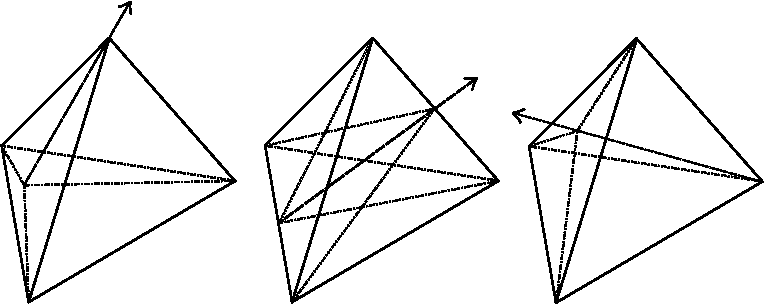
\includegraphics[width=1.0\textwidth]{chapters/theory/figures/CT_configurations.pdf}
  \caption{Potential Characteristic Tetrahedron (CT) configurations for non-planar angular direction.}
  \label{fig:non_planar_CTs}
\end{figure}

The first standard configuration involves a single incoming face and three outgoing faces with respect to the angular direction of the particle flow.
To apply the \ac{AHOT-C-UG} formalism to this tetrahedron, we split it into three CTs, thus allowing the computation of the angular flux over each CT and its outgoing face via the short characteristics equations.

The second standard configuration involves two incoming faces and two out-going faces with respect to the angular direction.
Unlike the previous standard configuration, it is necessary to determine both incoming and outgoing position vectors, in order to split the tetrahedron.
These vectors, analogous to the first standard configuration, are defined with respect to the global coordinate system.
In order to determine the characteristic length $\tau$, the arbitrary tetrahedron can be mapped into a normalized tetrahedron and the characteristic length can be determined based on the local angular direction.

The determination of the characteristic length involves the selection of a particular set of equations from the set of equations relating the global and local coordinate systems.
The local coordinate system can provide the specific values that are needed to determine the characteristic length.
In order to derive the formulas for $\tau$, it is necessary to consider every potential case in the normalized coordinate system.

The final standard configuration involves three incoming faces and a single outgoing face with respect to the angular direction.
In order to split such tetrahedron into CTs, it is necessary to determine the incoming position vector.
It is worth noting that this particular case is identical to the standard configuration 1 with the “in” and “out” designations for the corresponding position vectors interchanged.

In the event that the particle flight direction, $\vec{\Omega}$, is co-planar with one of the original tetrahedron's faces, or coincident with one of its edges the resulting set of potential CT splits is illustrated in \ref{fig:planar_CTs}.

\begin{figure}[th]
  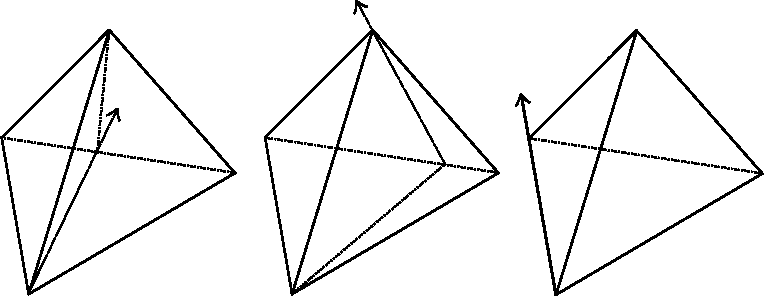
\includegraphics[width=1.0\textwidth]{chapters/theory/figures/CT_simplified.pdf}
  \caption{Simplified Characteristic Tetrahedron (CT) configurations for planar coincidental angular direction.}
  \label{fig:planar_CTs}
\end{figure}

The first simplified configuration involves two incoming faces and a single outgoing face with respect to the angular direction.
To split the cell, it is necessary to determine the outgoing position vector, which is the projection of the incoming vertex along the local angular direction to the outgoing face.
It is worthwhile to note that this particular case is identical to the standard configuration 2 with two instead of three constituent CTs.

The second simplified configuration involves one incoming face and two out-going faces with respect to the angular direction.
In order to split the cell into CTs, it is necessary to determine the incoming position vector, which is the projection of the outgoing vertex backwards along the angular direction to the incoming face.

The third simplified configuration involves a single incoming face and a single outgoing face.
This particular case occurs when the angular direction $\vec{\Omega}$ is parallel to exactly one edge of the arbitrary tetrahedron.
In this case, the arbitrary tetrahedron reduces to a CT and as such, it does not require any splitting.
This simplified configuration rarely occurs in actual applications, since the generation of the mesh and the selection of the angular quadrature are performed independently.
However, this configuration is also particularly important due to the fact that the discrete-ordinates solution being approximated by the \ac{AHOT-C-UG} over the discrete mesh will be smooth, since all potential discontinuities or so-called ‘singular characteristics’~\cite{Duo2009} will lie along the no-flow faces of the subject tetrahedrons, and thus they make no contribution to the incoming and outgoing angular fluxes over a given cell.
This feature of the discrete problem, in which high-order convergence may be observed, is attained provided that the tetrahedral grid is constructed in such a way that every cell has at least one side that is parallel to the particle flow angular direction.
This type of mesh generation strategy is termed "aligned mesh".

With regards to implementation into \ac{THOR}, an algorithm that determines the applicable CT configurations with respect to a given cell's orientation is devised by simply testing the number of incoming and outgoing cell faces.
Since the unstructured nature of the geometric description makes it impossible to determine \textit{a priori} the sweeping order of the mesh in the context of a single inner iteration, each cell is examined throughout the mesh-sweep process to determine the applicable CT configuration.
This enables locally solving the moments-balance and Short Characteristics equations simultaneously for each resulting CT, then the computed values are combined into face- and cell-moments of the angular flux valid for the original tetrahedral cell.
Hence, the information regarding the number of incoming and outgoing faces is determined on the fly and need not be stored thus relieving the memory storage burden.

\section{The \ac{AHOT-C-UG} Formulation}

The \ac{AHOT-C} formulation in two-dimensional Cartesian geometry~\cite{Azmy1992} involved the derivation of two fundamental sets of equations for each cell:
\begin{enumerate}
    \item The arbitrary-order balance equation over the cell, that relates the angular flux face-moments and distributed source cell-moments to the cell-moments of the angular flux.
    \item The arbitrary-order characteristic relation, that relates the angular flux incoming face-moments and distributed source cell-moments to the angular flux outgoing face-moments.
\end{enumerate}
An analogous approach is adopted in \ac{AHOT-C-UG}, except for the fact that the quantities of interest are defined in a transformed local coordinate system that does not leave the discrete-variable transport operators invariant, and as such requires a sequence of transformations in order to obtain discrete-variable expressions for the face- and cell-moments of the angular flux.
These transformation procedures allow for the expansion of the angular flux and the source to be represented in the local cell and CT coordinate system, thus simplifying the final set of equations that are implemented in \ac{THOR}.
It is important to note that none of these transformations introduce any additional approximation to the \ac{AHOT-C-UG} approach.
In order to develop these transformations, first it is necessary to define the face- and cell-moments and their accompanying basis functions.

\subsection{Polynomial Basis Function Expansion}

Let $B_{\vec{i}} (\vec{r})$ denote a polynomial basis function of order $\vec{i} = \{ i_j,j=1,2,3 \}$, where the $i_j$ satisfy the conditions $0 \leq i_1 + i_2 + i_3 \leq \Lambda '$ if a ‘complete’ basis is used or the conditions $0 \leq i_j \leq \Lambda , j = 1, 2, 3$ if a ‘double’ Pascal tetrahedron is used, in which case all mixed (or cross) moments that satisfy the corresponding conditions are retained by the expansion.
In both cases, $\Lambda$, and $\Lambda '$ denote the highest order of the polynomial basis, and thus determines the spatial expansion order of the method.
The basis functions for \ac{AHOT-C-UG} in the cell coordinate system is the monomial basis

\begin{equation} \label{eq:cell_basis}
    B_{\vec{i}} (\vec{u}) = u_1^{i_1} u_2^{i_2} u_3^{i_3}
\end{equation}

and, similarly, in the cell-face coordinate system the basis function is the monomial

\begin{equation} \label{eq:face_basis}
    B_{\vec{i}^F} (\vec{u}^F) = ( u_1^F )^{i_1^F} ( u_2^F )^{i_2^F}
\end{equation}

In general, the cell-moments in the global coordinate system are defined by

\begin{equation} \label{eq:cell_moments}
    G_{\vec{i}} \equiv \frac{1}{V} \int_{V} dV B_{\vec{i}} (\vec{r}) g(\vec{r})
\end{equation}

\noindent where $g( \vec{r} ) = \psi_n (\vec{r} ), \phi ( \vec{r} )$, or $S( \vec{r})$, and $V$ is the cell volume.
The cell face- or area-moments in the global coordinate system are defined in a similar manner

\begin{equation} \label{eq:face_moments}
    G_{\vec{i}}^F \equiv \frac{1}{A^F} \int_{A^F} dA^F B_{\vec{i}^F} (\vec{r}^F) g(\vec{r}^F)
\end{equation}

\noindent where $A^F$ is the area of the subject cell face.
The integrals in the global coordinate system are better evaluated in the cell coordinate system in order to avoid large values of the spatial-variable arguments in the former that might lead to poor numerical precision in the computed quantities.
Unlike the case of orthogonal functions in structured geometries, in which basis functions such as Legendre polynomials are used in rectangular cells, the use of monomials requires the solution of a linear system of equations in order to obtain the expansion coefficients of the projected functions.
Note that using orthogonal bases in unstructured grids is futile since there is no expectation of orthogonality in these configurations.
For instance, if the function $g( \vec{r}) $ in Eq. \ref{eq:cell_moments} is expanded locally into the set of basis functions defined in Eq. \ref{eq:cell_basis}

\begin{equation} \label{eq:g_expansion}
    g (\vec{u}) = \sum_{\vec{i}=0}^{\Lambda} g_{\vec{i}} B_{\vec{i}} (\vec{u})
\end{equation}

\noindent then the vector $\bold{G}$ whose $\vec{i}^{th}$ element is given by Eq. \ref{eq:cell_moments}, and packing the scalar expansion coefficients $g_{\vec{i}}$ into the vector $\bold{g}$ we can relate these two vectors by taking the $\vec{i}^{th}$ moment of Eq. \ref{eq:g_expansion} via,

\begin{equation} \label{eq:expansion_coefficients}
    \bold{G} = \boldsymbol{M} \bold{g}
\end{equation}

\noindent In Eq. \ref{eq:expansion_coefficients} matrix $\boldsymbol{M}$ is the tensor product of the monomial basis (also known as the mass matrix in finite element methods), that is defined in the following manner

\begin{equation} \label{eq:mass_matrix}
    \boldsymbol{M} \equiv 6 \int_{0}^{1} du_1 \int_{0}^{u_1} du_2 \int_{0}^{u_2} du_3 B_{\vec{i}} B_{\vec{i}}^{\boldsymbol{T}}
\end{equation}

\noindent where $\boldsymbol{M}$ and $B_{\vec{i}} B_{\vec{i}}^{\boldsymbol{T}}$ are matrices of order $\Lambda$ or $\Lambda '$, for double Pascal or complete basis, respectively, and the superscript $\boldsymbol{T}$ denotes the transposed vector.
In Eq. \ref{eq:expansion_coefficients} the components of $\bold{g}$ represent the known or unknown local expansion coefficients of the function $g( \vec{r})$ if $g$ is the fixed source or the angular flux, respectively.

The choice of monomials as basis functions was motivated by previous experience, namely the formulation of \ac{AHOT-C-UG} presented in~\cite{Azmy2001} that used this basis, as well as simplicity since in this basis the coordinate transformations become relatively straightforward to generalize to an arbitrary expansion order.
In addition, the overall results of early investigations reported in~\cite{FerrerPhD} illustrated insensitivity of the computed results to the particular choice of a different polynomial basis, such as a hierarchical basis~\cite{Wang2009}, as long as the basis spans the same exact function space~\cite{Adams2001}.
While the structured grid-based formulation of \ac{AHOT-C} used Legendre polynomials as basis  functions, which retained mixed product terms, this is not generally a requirement.
Due to the generality of the \ac{AHOT-C-UG} formalism, it is possible to experiment with both types of basis function expansions.

The use of a ‘mixed’ or incomplete basis expansion introduces an additional complication that is not encountered in the case of a complete basis.
This additional complication stems from the fact that, given a particular incoming and outgoing direction in the cell coordinate system, the evaluation of the angular flux moments over the CT volume and outgoing face in the CT coordinate system must be consistent with the expansion in the cell coordinate system.
For example, consider the $\Lambda = 1$ expansion, $\{1, x, y, z, xy, xz, yz, xyz \}$, over a normalized tetrahedron.
Let $x = u_1, y = u_2$, and $z = u_3$ and consider the case in which the outgoing angular flux, determined by the local angular direction, exits the face defined by $u_3 = 0$, as represented by the CT located inside the first tetrahedron on the left in Fig. \ref{fig:non_planar_CTs}.
The basis functions used to represent the angular flux in the cell coordinate system over the outgoing face become $\{ 1, x, y, xy \}$.
If the incoming angular flux moments and distributed source are simply transformed to the local CT coordinate system based on an incomplete expansion, such as $\{ 1, x, y, z, xy, xz, yz, xyz \}$ under the assumption that $x = q_1, y = q_2$, and $z = q_3$, then the outgoing face-moments computed by the CT will automatically assume, by convention, that the outgoing angular flux exists the face defined by $u_3 = u_2$, and thus assumes that the basis expansion over the outgoing CT face is given by $\{ 1, x, y, xy, y^2, xy^2 \}$, which is clearly different from in the cell coordinate system.

In order to maintain the correct orientation, the computation of the spatial moments of the angular flux over the outgoing face and volume has to be  performed in tandem with the coordinate transformation.
This peculiarity does not arise in a complete expansion, since in the case of $\Lambda ' = 1$ the expansion is $\{ 1, x, y, z \}$ which, when evaluated over the outgoing face in the cell coordinate system is $\{ 1, x, y \}$, and in the CT coordinate system is $\{ 1, x, y \}$, both of which are clearly compatible with each other.

\subsection{Transformation of Cell to CT Source Distribution}

In order to simplify the computation of the outgoing face moments of the angular flux via the characteristic relation, the source moments and expansion coefficients over the cell must be transformed into the CT coordinate system.
In accordance with Eq. \ref{eq:expansion_coefficients}, the moments and expansion coefficients for the source distribution in the cell and CT coordinate systems are related via

\begin{equation}
    \bold{S} = \boldsymbol{M} \bold{s}
\end{equation}

and

\begin{equation} \label{eq:CT_moments2expansion}
    \bold{S}^v = \boldsymbol{M}^v \bold{s}^v
\end{equation}

\noindent respectively, where the $v$ superscript implies CT coordinate system, and the $\vec{i}^{th}$ elements of $\bold{s}$ and $\bold{s}^v$ is $s_{\vec{i}}$ and $s_{\vec{i}}^v$, respectively, with analogous relationships for the moment vectors $\bold{S}$ and $\bold{S}^v$.
The distributed source within a CT is equal to the cell source distribution over the volume of the tetrahedron with respect to the global coordinate system, $S(\vec{r}) = S^v(\vec{r})$, where $S^v$ is the distributed source over the volume of the CT.
Thus, the spatial moments of the source over the CT is obtained by integrating the product of the corresponding monomial and the cell distributed source over the domain of the CT, i.e.,

\begin{equation} \label{eq:defineSv}
    S^{v}_{\vec{i}} = \frac{1}{V^v} \int_{V^v} d V^v B_{\vec{i}}^{v} (\vec{r}) S (\vec{r})
\end{equation}

Since the distributed source moments are expressed in the cell coordinate system, Eq. \ref{eq:defineSv} must reflect this coordinate transformation.
Substituting Eq. \ref{eq:g_expansion}, with $g( \vec{u} ) = S( \vec{u} )$, into Eq. \ref{eq:defineSv} and evaluating the expression in the CT coordinate system yields the following relation between the CT source moments, $\bold{S}^{v}$, and the cell source expansion coefficients, $\bold{s}$,

\begin{equation}
    \bold{S}^{v} = \boldsymbol{P} \bold{s}
\end{equation}

\noindent where matrix $\boldsymbol{P}$ contains the basis product integration.
This matrix allows the transformation of the distributed source expressed via expansion coefficients over a cell into a source distribution expressed via CT moments over a CT.
However, the explicit evaluation of the matrix $\boldsymbol{P}$ requires careful consideration.
The cell moments of the distributed source are expressed in the cell coordinate system, while the CT moments of the distributed source are expressed in the CT coordinate system.
In order to correctly evaluate matrix $\boldsymbol{P}$, the integration must be performed in the CT coordinate system and the source expansion coefficients in the cell coordinate system must be transformed into the CT coordinate system.

In order to derive the characteristic equation, and determine the outgoing face angular fluxes, two more procedures are required.
First, the upstream cell’s outgoing face angular flux moments from a neighboring cell must be transformed into downstream incoming face moments.
Second, it is necessary to transform the incoming face angular flux moments into CT face angular moments.
Once these procedures are applied to the specified moments, the characteristic relation can be derived in the CT coordinate system.

\subsection{Upstream to Downstream Face Angular Flux Moment Transformation}

Analogous to the source distribution, the upstream/downstream face angular flux moments, denoted by the vectors $\bold{\Psi}^{F,up/down}$, and the expansion coefficients, denoted by the vector $\boldsymbol{\psi}^{F,up/down}$, are related via,

\begin{equation}
    \bold{\Psi}^{F,up} = \boldsymbol{M}^F \boldsymbol{\psi}^{F,up}
\end{equation}

\begin{equation}
    \bold{\Psi}^{F,down} = \boldsymbol{M}^F \boldsymbol{\psi}^{F,down}
\end{equation}

\noindent where the $\vec{i}^{th}$ element of each of these vectors corresponds to the $\vec{i}^{th}$ moment and $\vec{i}^{th}$ expansion coefficient, respectively, of the corresponding quantity.
The matrix $\boldsymbol{M}^F$ is defined in analogy to Eq. \ref{eq:mass_matrix}

\begin{equation} \label{eq:defineMF}
    \boldsymbol{M}^F \equiv 2 \int_{0}^{1} du_1^F \int_{0}^{u_1^F} du_2^F B_{\vec{i}^F}^F {B_{\vec{i}^F}^F}^{\boldsymbol{T}}
\end{equation}

\noindent where $\vec{i}^F = \{ i_1^F , i_2^F \}$ and the components of this vector satisfy either $0 \leq i_1^F + i_2^F \leq \Lambda '$ or $0 \leq i_1^F + i_2^F \leq 2 \Lambda$, depending on the expansion method.
In order to relate the upstream and downstream moments, which may not be expressed in the same face coordinate system, we assume that the angular flux evaluated on a given face in the global coordinate system is continuous across that face, i.e. no jump conditions on cell interfaces, $\psi^{F,up} ( \vec{r}) = \psi^{F,down} ( \vec{r})$, such that $\vec{r}$ is a point on the face separating the indicated tetrahedra.
Thus, the spatial moments of the downstream face angular flux become

\begin{equation} \label{eq:Psidown}
    \Psi_{\vec{i}^F}^{F,down} = \frac{1}{A^F} \int_{A^F} dA^F B_{\vec{i}^F}^{F,down} (\vec{r}) \psi^{F,up} (\vec{r})
\end{equation}

Since the upstream face moments are expressed in the cell face coordinate system, Eq. \ref{eq:Psidown} must reflect this coordinate transformation.
Substituting Eq. \ref{eq:g_expansion}, with $g( \vec{u} ) = \psi^{F,up} ( \vec{u} )$ and $B_{\vec{i}} ( \vec{u } ) = B_{\vec{i}^F}^{F,down} (\vec{u})$, into Eq. \ref{eq:Psidown} yields the following relation between the moments, as evaluated in the downstream cell face coordinate system

\begin{equation} \label{eq:down2up}
    \bold{\Psi}^{F,down} = \boldsymbol{T} \bold{\Psi}^{F,up}
\end{equation}

\noindent where matrix $\boldsymbol{T}$ contains elements representing the basis product integration.
This matrix allows the transformation of upstream face moments in the upstream coordinates system into downstream moments in the downstream coordinate system.

\subsection{Incoming Angular Flux Cell and CT Transformation}

In order to apply the characteristic relation, an additional transformation is introduced to map the incoming angular flux moments from the cell face coordinate system to the CT face coordinate system.
The development of this transformation is rather similar to the development of the transformation of the distributed source.
The incoming face angular flux moments and expansion coefficients over the cell and CT, respectively, are related via the following expressions,

\begin{equation}
    \bold{\Psi}^{F,in} = \boldsymbol{M}^F \boldsymbol{\psi}^{F,in}
\end{equation}

\begin{equation} \label{eq:Psi.f.in}
    \bold{\Psi}^{f,in} = \boldsymbol{M}^f \boldsymbol{\psi}^{f,in}
\end{equation}

\noindent where $\boldsymbol{M}^f$ is defined in a similar manner to Eq. \ref{eq:defineMF}

\begin{equation}
    \boldsymbol{M}^f \equiv 2 \int_{0}^{1} dq_1^f \int_{0}^{q_1^f} dq_2^f B_{\vec{i}^f}^f {B_{\vec{i}^f}^f}^{\boldsymbol{T}}
\end{equation}

\noindent where $\vec{i}^f = \{ i_1^f , i_2^f \}$ and the components of this vector satisfy either $0 \leq i_1^f + i_2^f \leq \Lambda '$ or $0 \leq i_1^f + i_2^f \leq 2 \Lambda$, depending on the expansion method.
Again we assume no jump conditions on tetrahedron faces so that in the global coordinate system we may write $\psi^{f,in} ( \vec{r} ) = \psi^{F,in} ( \vec{r} )$.
The spatial moments of the CT incoming face angular flux in terms of the \textit{cell} face incoming angular flux expansion, are expressed by the following relation

\begin{equation} \label{eq:Psi.f.in.element}
    \Psi_{\vec{i}^f}^{f,in} = \frac{1}{A^f} \int_{A^f} dA^f B_{\vec{i}^f}^{f,in} (\vec{r}) \psi^{F,in} (\vec{r})
\end{equation}

Substituting the explicit expansion for $\psi^{F,in} (\vec{r})$ in the cell face coordinate system into Eq. \ref{eq:Psi.f.in.element} yields the following relation between the moments written in vector form, with the elements interpreted as before,

\begin{equation}
    \bold{\Psi}^{f,in} = \boldsymbol{p}^F \boldsymbol{\psi}^{F,in}
\end{equation}

\noindent where matrix $\boldsymbol{p}^F$ contains the basis product integration element by element.
This matrix allows the transformation of incoming face moments in the cell coordinate system into incoming moments in the CT coordinate system.
\textbf{Question:} \textbf{If RHS of above Eq is moments, shouldn't it be $\Psi$?}

\subsection{Face Moments of the Arbitrary-Order Characteristic Relation}

The outgoing angular face flux for a CT, assuming known incoming and distributed source spatial moments in the CT coordinate system, can be computed using the characteristic relation.
The characteristic relation originates from the exact local inversion of the streaming-plus-collision operator of the transport equation along the angular direction.
The general characteristic relation in the CT coordinate system for the case of isotropic fixed source is

\begin{equation} \label{eq:CC.relation}
    \psi^v(\vec{r}^{in} + t \hat{\Omega} ) = \psi^{f,in} (\vec{r}^{in}) e^{- \sigma_T t} + \int_{0}^{t} dt' S^v (\vec{r}^{in} + t' \hat{\Omega}) e^{- \sigma_T (t - t')}, 0 \leq t \leq \tau ,
\end{equation}

\noindent where $t$ is the physical distance measured along the characteristic from the incoming point $\vec{r}^{in}$, $\tau$ is the physical extent of the cell along $\hat{\Omega}$, and the superscript $v$ denotes the selected CT domain within the cell.
Evaluating Eq. \ref{eq:CC.relation} on the outgoing face of the CT then taking moments in the CT coordinate system yields

\begin{equation}
    \bold{\Psi}_{\vec{i}^f}^{f,out} = \frac{1}{A^f} \int_{A^f} dA^f B_{\vec{i}^F}^{F,out} \psi^{f,out} (\vec{r} )
\end{equation}

\noindent from which moments on the cell’s outgoing face, in the cell coordinate system, are accumulated via

\begin{equation}
    \bold{\Psi}_{\vec{i}^F}^{F,out} = \sum_f \frac{A^f}{A^F} \bold{\Psi}_{\vec{i}^f}^{f,out}
\end{equation}

Recalling Eqs. \ref{eq:Psi.f.in} and \ref{eq:CT_moments2expansion}, the following expression for the outgoing CT face moments is obtained

\begin{equation}
    \bold{\Psi}_{\vec{i}^f}^{f,out} = \boldsymbol{F} \boldsymbol{\psi}^{f,in} + \boldsymbol{V} \bold{s}^v
\end{equation}

\noindent where the elements of matrices $\boldsymbol{F}$ and $\boldsymbol{V}$ represent the integration of the exponential functions and basis product in the CT coordinate system, and the elements of the  vectors $\boldsymbol{\psi}^{f,in}$ and $\bold{s}^v$ are $\psi_{\vec{i}}^{f,in}$ and $s_{\vec{i}}^v$, respectively.

\subsection{Incoming and Outgoing Angular Flux Cell Transformation}

Once the outgoing face moments in the cell face coordinate system are computed, they must be transformed into the cell coordinate system via the relation,

\begin{equation}
    \bold{\Psi}^F = \boldsymbol{T}^F \boldsymbol{\psi}^F
\end{equation}

\noindent where the matrix $\boldsymbol{T}^F$ contains the basis product integration.
Note that the evaluation of $B_{\vec{i}} ( \vec{u})$ will depend on the face under consideration.

\subsection{The Arbitrary Order Characteristic Relation}

Given a known distributed source and incoming face angular flux, the spatial moments of the angular flux over the CT can be computed via the characteristic relation.
As shown in the previous section, the characteristic relation exactly satisfies the arbitrary order balance equation.
Thus, the spatial moments computed from either equation will comprise the same solution.
However, due to the fact that finite arithmetic precision can be affected by the buildup of round-off error, two equivalent mathematical statements may yield either slightly or significantly different results.
In the case of the spatial moments of the angular flux, rather large discrepancies were observed as the cells were made less absorbing.
Conversely, in the case of highly absorbing cells, the discrepancies between the results obtained via the characteristic and the balance equations formulations diminished, hence it was possible to verify numerically the equivalence between the two formulations.

In this section the procedure for computing the spatial moments of the angular flux from the characteristic equation is reviewed and all relevant relations are derived.
Recall that in the CT coordinate system, the characteristic relation is given by Eq. \ref{eq:CC.relation}.
Instead of obtaining the spatial moments in the CT coordinate system, the moments in the $cell$ coordinate system will be directly obtained from the characteristic equation,

\begin{equation}
    \bold{\Psi} = \sum_v \left( \frac{V^v}{V} \right) \bold{\Psi}^v
\end{equation}

\noindent where the $\vec{i}^{th}$ element of the vector $\bold{\Psi}^v$ is computed by,

\begin{equation} \label{eq:psiv}
\begin{split}
    \psi^v_{\vec{i}} & = \frac{1}{V^v} \int_{V^v} dV^v B_{\vec{i}} ( \vec{r} ) \psi^v ( \vec{r} ) \\
    & = 6 \int_0^1 dq_1 \int_0^{q_1} dq_2 \int_0^{q_2} dq_3 B_{\vec{i}} ( \vec{u} ) \psi^v ( \vec{q} )
\end{split}
\end{equation}

By substituting Eq. \ref{eq:CC.relation} into Eq. \ref{eq:psiv}, the following expression for the CT spatial moments is obtained,

\begin{equation}
    \bold{\Psi}^v = \boldsymbol{F}^v \boldsymbol{\psi}^{f,in} + \boldsymbol{V}^v \bold{s}^v
\end{equation}

Note that the basis multiplying the characteristic equation is in the cell coordinate system.
This concludes the introduction and development of the necessary equations and relations needed to apply the \ac{AHOT-C} formalism to unstructured tetrahedral grids.
The only outstanding issue that remains unresolved is the explicit computation of the integral kernels.
In the next section the evaluation of these integral kernels will be discussed and series expansions will be derived in order to obtain stable expressions suitable for computing the spatial moments as the cells become optically thin.

\section{Series Expansion of Integral Kernels in Arbitrary-Order Characteristics Relation}

The expressions derived for the CT, that relate the outgoing face-moments and cell volume-moments of the angular flux via the characteristic relation, can be evaluated analytically by repeatedly applying integration by parts to the basis functions.

In order to derive the series expressions for the outgoing face moments of the angular flux, the exponential function appearing in the integrand is expanded locally into a Taylor series,

\begin{equation} \label{eq:TaylorExp}
    e^{- \epsilon q^f_2} = \sum_{n=0}^{\infty} \frac{(-1)^n}{n!} \epsilon^n \left( q_2^f \right) ^n
\end{equation}

\noindent then substituted into the integral expression to yield,

\begin{equation}
    \Gamma_{\gamma_1^f ,\gamma_2^f} ( \epsilon ) = \sum_{n=0}^{\infty} \frac{(-1)^n}{n!} \frac{\epsilon^n}{( \gamma_1^f + \gamma_2^f +n+2) (\gamma_2^f +n+1)}
\end{equation}

In a similar development, the exponential function in the cell volume is split into the product of two exponentials, where the first term has the Taylor expansion Eq. \ref{eq:TaylorExp}, and the second term yields,

\begin{equation}
    e^{\epsilon q_2^f} = \sum_{n=0}^{\infty} \frac{1}{n!} \left( q_2^f \right) ^n
\end{equation}

\noindent These two Taylor expansions are then substituted into the corresponding integral expression in order to obtain the following series representation,

\begin{multline}
    \Gamma_{\gamma_1 ,\gamma_2 ,\gamma_3} ( \epsilon ) = \sum_{n=0}^{\infty} \sum_{m=0}^{\infty} \frac{(-1)^m \epsilon^{n+m}}{n! m!} \\
    \frac{1}{( \gamma_1 + \gamma_2 + \gamma_3 +n+m+3) ( \gamma_2 + \gamma_3 +n+m+2) (\gamma_3 +n+1)}
\end{multline}

In order to derive the series expressions for the spatial moment integrals of the angular flux over the cell volume, the exponential function for the incoming face angular fluxes for the the spatial moments over the volume is expanded into a polynomial series in a similar fashion to the previous procedure,

\begin{equation}
    e^{- \epsilon q^f_3} = \sum_{n=0}^{\infty} \frac{(-1)^n}{n!} \epsilon^n \left( q_3 \right) ^n
\end{equation}

\noindent that is then substituted into the corresponding integral relation in order to obtain the following expressions,

\begin{multline}
    \Gamma^v_{\gamma_1 ,\gamma_2 ,\gamma_3} ( \epsilon ) = \sum_{n=0}^{\infty} \frac{(-1)^n \epsilon^{n}}{n!} \\
    \frac{1}{( \gamma_1 + \gamma_2 + \gamma_3 +n+3) ( \gamma_2 + \gamma_3 +n+2) (\gamma_3 +n+1)}
\end{multline}

\begin{multline}
    \Gamma^v_{\gamma_1 ,\gamma_2 ,\gamma_3 ,\gamma'_3} ( \epsilon ) = \sum_{n=0}^{\infty} \sum_{m=0}^{\infty} \frac{(-1)^m \epsilon^{n+m}}{n! m!} \frac{1}{( \gamma_1 + \gamma_2 + \gamma_3 + \gamma'_3 +n+m+4)}\\
    \frac{1}{( \gamma_2 + \gamma_3 + \gamma'_3 +n+m+3) ( \gamma_3 + \gamma'_3 +n+m+2) ( \gamma'_3 +n+1)}
\end{multline}

In summary, the integral kernels contained in the arbitrary-order characteristic equations were expanded using a Taylor series of the exponential functions and their corresponding integrals were evaluated on a term by term basis.
These integral kernels, that are now represented by local series expansions, enable computing the contribution of the incoming angular fluxes and distributed source to the outgoing face moments and spatial moments of the angular flux over the given cell.
It is important to note that this local expansion treatment resolves previously reported instabilities of the computational method in the limit of thin cell and with increasing spatial approximation order~\cite{Azmy2001}.
Evidence to this statement is provided by numerical experiments that were reported elsewhere.

This concludes the development of a robust \ac{AHOT-C-UG} methodology for the solution to the discrete-ordinates approximation to the transport equation
on three dimensional tetrahedral grids.